\chapter{High-Precision Distance Moduli from Single-Epoch Spectrophotometry Using Deep Learning}
\label{chap:nn_twins}

\section{Introduction}
\label{sec:nn_twins_intro}
Observations Type Ia supernovae (SNe Ia) continue to serve as  one of the strongest tools for measuring cosmological distances and inferring the expansion history of the universe. Their strength as distance indicators relies on their relative homogeneity in absolute brightness. Much effort has gone into improving how standard these standard candles are, using empirical correlations between observable properties and absolute luminosity to correct differences in peak brightness based on measured differences in these other properties.

Without any additional corrections, SNe Ia peak magnitudes are consistent to within $\sim0.4$ magnitudes. Initially, SNe Ia were standardized using the decay time of their light curves \citep{phillips_absolute_1993}. Later, additional correlations were found between brightness and broadband $B-V$ colors \citep{riess_precise_1996, tripp_two-parameter_1998}. Including these corrections decreases the spread of the corrected peak brightnesses to the level of $\sim 0.15$ magnitudes.

Today, most cosmology analyses use parametrized models of the underlying spectral energy distribution of SNe Ia. The most common model, SALT2 \citep{guy_salt2_2007, betoule_improved_2014} parametrizes the full spectral evolution of SNe Ia with two components: $x_1$, which mimics the light curve width used in original standardization processes, and $c$ which captures the color differences due to both intrinsic variation and dust in the line of sight. These two corrections standardize the SNe Ia brightnesses to 0.14 mag. SNEMO, introduced in \cite{saunders_snemo_2018}, extends the SALT2-like standardization methodology by including additional degrees-of-freedom in the model in order to describe the variation in supernova spectral time-series data. The 7-component SNEMO7 model is able to standardize supernova magnitudes to 0.113 mag.

Much work has also gone into understanding ways to standardize supernovae using their spectra, rather than exclusively using broadband light curves. Some studies have identified particular regions of the spectra that can be used to standardize their brightness. \citet{nugent_evidence_1995} identified that the ratio of the equivalent widths of \ion{Si}{2} 5972~\AA\ and \ion{Si}{2} 6355~\AA\ are strongly related to light curve width, and \citet{bailey_using_2009} found that the flux ratios between specific wavelengths can be used for standardization. \citet{nordin_understanding_2018} uses specific spectral features in the near-UV to standardize. \cite{leget_sugar_2020}, built SUGAR, an SED model based on a PCA decomposition of a number of spectral features across a wide range of wavelengths.

\citet{fakhouri_improving_2015} took a slightly different approach, directly comparing spectra near maximum brightness to one another to identify pairs of ``twins". On average, the best 15\% of twins differ in magnitude by only 0.08 mag, making this twinness methodology one of the best methods for standardizing supernova magnitudes. \citet{boone_twins_2020a} (hereafter \citetalias{boone_twins_2020a}) aimed to elucidate the mathematical structure underlying this twinning method by applying manifold learning techniques to identify a low-dimensional representation of the twinness space. Using projections into this lower dimensional space, \citet{boone_twins_2020b} (hereafter \citetalias{boone_twins_2020b}) was then able to model the necessary corrections to the supernova magnitudes based on these projections, standardizing supernovae with an RMS error of $0.101 \pm 0.007$ mag.

However, the \citetalias{boone_twins_2020b} standardization analysis requires at least one spectrum in a narrow phase range around maximum brightness. The goal of the work we present here is two-fold: first to extend the use of the twins embedding standardization to a wider range of phases, and second to create a generative model that can be used in simulations or fitting lower-resolution spectroscopy or broadband photometry. The first goal is accomplished with a model that we refer to throughout the work as \stoe, which takes a spectrum and predicts its phase along with the extinction parameter and twins embedding coordinate of the supernova that spectrum was taken from. To accomplish the second goal, we build a model that we call \etos{} to predict the spectral energy distribution (SED) of a supernova given its location in the twins embedding space and dust extinction parameter, up to a gray magnitude offset.

Both of these models are built using deep neural networks. This work is not the first application of deep learning to problems relevant to Type Ia supernovae or supernova cosmology. \citet{sasdelli_exploring_2016} used an unsupervised deep autoendoder network to model the intrinsic spectral diversity of SNe Ia. \citet{muthukrishna_dash_2019} used supervised deep learning to automate the classification of transient types, redshifts, ages, and host morphologies based on spectra. Both of these models are used only in spectroscopic classification -- neither makes an attempt to improve the standardization of the supernovae under study. \citet{stahl_deepsip_2020} is the first work to use deep learning to predict light curve properties that can be used in standardization from spectra, using deep convolutional neural networks to predict the phase and light curve shape parameter $\Delta m_{15}$. This network could predict $\Delta m_{15}$ to within 0.056 magnitudes, which propagates to a standardized magnitude error (using the Phillips relation of \citet{phillips_absolute_1993}) of approximately 0.151 mag. Our work is motivated by a desire to combine the success of deep learning methods in identifying valuable non-linear relationships between supernova spectra and low-dimensional representations of their behavior, with the success of the \citetalias{boone_twins_2020a} and \citetalias{boone_twins_2020b} analyses in standardizing supernovae using these low-dimensional representations. 

We begin in Section \ref{sec:boone_summary} by summarizing the steps of the twins embedding analysis in more detail. In Section \ref{sec:nn_twins_data}, we explain the data set used throughout our analysis. In Section \ref{sec:model}, we present the neural network architectures used for both the models, as well as our techniques for finding optimal model hyperparameters. We examine how well our neural network is able to recover the twins embedding coordinates and how the embedding coordinate errors propagate to standardization errors in Section \ref{sec:spec2embed_results}. In Section \ref{sec:embed2spec_results}, we evaluate the performance of the \etos{} model. We conclude in Section \ref{sec:nn_twins_conclusions} with some suggestions for further analyses using these tools.

\section{The Twins Embedding Analysis} \label{sec:boone_summary}
The following is a summary of the main methods and results of the twins embedding analyses presented in \citetalias{boone_twins_2020a} and \citetalias{boone_twins_2020b} that are needed to understand the work presented here. Full details can be found in the cited papers. The twins embedding analysis consists of four main parts: the differential time evolution model, the ``read between the lines" analysis, the Isomap embedding analysis, and the Gaussian process model of the relationship between the color and embedding coordinates of a supernova and its deviation in brightness on the Hubble diagram. The first three subanalyses are presented in \citetalias{boone_twins_2020a}, while the final portion is presented in \citetalias{boone_twins_2020b}.

The differential time evolution model interpolates all observed spectra from $-5$ to $+5$ days after maximum brightness to the time of maximum brightness. The model takes advantage of the fact that while the spectra of each supernova can look quite different at maximum light, their differential evolution near maximum is remarkably similar. Additionally, because the differential evolution is being modeled, multiplicative effects on the spectrum (e.g. magnitude differences from distance uncertainties or color differences from dust extinction) have no effect on the model. The time evolution of the spectrum flux of each supernova is modeled as a quadratic function of the phase; this is an excellent approximation near maximum brightness, but breaks down beyond $\pm~5$ rest-frame days, motivating an alternate modeling methodology for phases outside of this quadratic regime.

With the interpolated at-maximum spectra in hand, the ``read between the lines" analysis (hereafter RBTL) is then used to describe the differences in brightness ($\Delta m$) and differential dust extinction parameter ($\Delta A_V$) between each spectrum and a mean spectrum. The mean spectrum is the weighted average of all of the at-max spectra, with the weights being determined by the simultaneously-fit intrinsic variation at each wavelength. This weighting scheme means that the model in effect uses only the regions of the spectrum that are most intrinsically standard to determine the magnitude heterogeneity and extinction of the supernovae. Using just the RBTL magnitude offsets without any additional corrections, the \sne are able to be standardized to within 0.131 mag. At this stage, though, some intrinsic variation in the spectra can be confused for extrinsic variation if this intrinsic variation looks like a difference in extinction or brightness. However, if we make the assumption that this variation also makes changes that can be measured from changes to spectral features, we can later correct for these differences. This motivates the final two subanalyses: the Isomap embedding and estimation of magnitudes using Gaussian process regression.

Isomap is a non-linear machine learning technique for finding approximately isometric low-dimensional embeddings of high-dimensional spaces. The \citetalias{boone_twins_2020a} analysis uses this algorithm on spectra that have been corrected for the brightness and color differences identified by the RBTL analysis, and so learns a low-dimensional representation of the intrinsic variation of at-max spectra. This embedding (the twins embedding) is three-dimensional, with coordinates labeled by ($\xi_1$, $\xi_2$, $\xi_3$). The twins embedding qualitatively reflects the diversity of \sn spectra, clustering objects with similar subclassifications together and pushing objects known to have peculiar subtypes (91T-like, 91bg-like, and 02cx-like) out to the periphery of the embedding space. 

The twins embedding coordinates can also be used to correct for the intrinsic contributions to the magnitude residuals from RBTL. \citetalias{boone_twins_2020b} presents a Gaussian process (GP) regression model to estimate the RBTL magnitude residual from the Isomap embedding coordinate. The GP allows us to capture non-linear relationships between the twins embedding coordinates and the magnitudes and also provides an estimate of the error. Mathematically, they model:
\begin{equation}
    \vec{m} \sim \mathcal{GP}\left(m_{\text{ref}} + \omega\Delta A_V, \mathbb{I}\cdot(\vec{\sigma}_{\text{pv}}^2 + \sigma_u^2) + K_{3/2}(\vec{\xi}, \vec{\xi}; A, l)\right)
\end{equation}
The $\omega\Delta A_V$ term and arbitrary $m_{\text{ref}}$ in the mean function corrects for the possibility of introducing a correlation between extinction and magnitude from an incorrect fiducial $R_V$. The correlation between embedding coordinate and magnitude is captured by a 3-dimension Mat\'{e}rn 3/2 kernel with length scale $l$ and amplitude $A$. The per-supernova uncorrelated errors from peculiar velocities enter into the model with through $\sigma_{\text{pv}}$. Any unexplained error (including systematic error from the analysis) is captured by $\sigma_u$, which is constant for all objects in the sample.

Using leave-one-out cross-validation, the full analysis is found to be able to standardize the studied sampled of SNe Ia with an RMS of $0.101 \pm 0.007$ mag. After accounting for the contributions from peculiar velocities, this RMS is reduced to $0.084 \pm 0.009$ mag.

Our first model, \stoe, seeks to mimic the first three subanalyses, taking a spectrum and determining its phase (in lieu of interpolating to maximum brightness), relative dust extinction parameter $\Delta A_V$, and twins embedding coordinate $(\xi_1, \xi_2, \xi_3)$ using a deep neural network. The final GP regression analysis step remains unchanged, but we examine the increase in residual spread from propagating the errors from replacing the RBTL and Isomap process with a neural network. Our second model, \etos, can be thought of as an inversion of the Isomap embedding analysis, taking the twins embedding coordinate and predicting the spectrum at any phase $p$, corrected for $\Delta m$ and $\Delta A_V$. The differences in magnitude and dust extinction can then be added using their known behavior. The result is a model that predicts the spectrum at a wide range of phases that takes $(\Delta m, \Delta A_V, \xi_1, \xi_2, \xi_3)$ as input.

\section{Data} \label{sec:nn_twins_data}
Both the twins embedding analysis and our work were trained using spectrophotometry from of the Nearby Supernova Factory (SNfactory) data set. All of the spectra were obtained with the Super Nova Integral Field Spectrograph (SNIFS; \cite{lantz_snifs_2004})  mounted on the University of Hawai`i 2.2-meter telescope on Maunakea. The spectra were reduced using the SNfactory data reduction pipeline (Ponder, et al. 2020, in preparation), calibrated via the process presented in \cite{buton_atmospheric_2013}, and host galaxy subtracted as described in \cite{bongard_3d_2011}. Reddening by Milky Way dust in the line of sight is removed assuming a Cardelli \citep{cardelli_relationship_1989} extinction law and using the dust maps from \cite{schlegel_maps_1998}.

After host galaxy subtraction and correction for Milky Way dust, we shifted the wavelengths of each spectrum in our analysis into the rest frame and rebinned the flux and flux variance onto a common wavelength grid from $3300 - 8600$~\AA\ with 1000~km/s-wide bins using \texttt{sncosmo}. This binning is identical to that used by \cite{fakhouri_improving_2015}, \cite{saunders_snemo_2018}, and \cite{boone_twins_2020a}. We also normalized the rebinned spectral flux and flux variance to a reference redshift of $z_\mathrm{ref}=0.05$ using
\begin{equation}
    F_\mathrm{rest} = F_\mathrm{obs} \left(\frac{1+z}{1+z_\mathrm{ref}}\right)\left(\frac{d_L(z_\mathrm{helio}, z_\mathrm{CMB})}{d_L(z_\mathrm{ref}, z_\mathrm{ref})}\right)^2 \times 10^{15}
    \label{eqn:idr_restframe}
\end{equation}
where $d_L(z_\mathrm{helio}, z_\mathrm{CMB})$ is the luminosity distance at redshift $z$, assuming a flat, $\Lambda$CDM cosmology with $H_0=70$~km~s$^{-1}$~Mpc$^{-1}$ and $\Omega_M=0.3$ for the heliocentric and CMB-frame redshifts:
\begin{equation}
    d_L(z_\mathrm{helio}, z_\mathrm{CMB}) = \frac{c}{H_0}(1+z_\mathrm{helio})\displaystyle\int_0^{z_\mathrm{CMB}} \frac{dz}{\sqrt{\Omega_M(1+z)^3 + (1-\Omega_M)}}.
\end{equation}
This normalization serves to adjust the observed magnitudes of every object in our sample to match the magnitudes they would have if they were all at the same reference redshift. The factor of $10^{15}$ in Eqn. \ref{eqn:idr_restframe} serves only to make the flux and variance values $\mathcal{O}(1)$ (in units of ergs~cm$^{-2}$~s$^{-1}$~\AA$^{-1}$). Note that in the redshift range of our sample, the difference between the fiducial cosmological model used and a pure Hubble law (i.e. a linear relationship between redshift and distance) is $\sim 0.01$ magnitudes. Thus, the analysis is insensitive to changes in the exact values of the cosmological parameters.

In addition to the spectral observations, the SNfactory pipeline synthesizes photometry for each of the observed SNe and uses these synthesized magnitudes to find the best-fit SALT2 model parameters $x_1$, $c$, and $m_B^*$ for each object, as well as an estimate of the time of maximum brightness $t_0$. The synthesized photometry SALT2 estimate of $t_0$ and the measured host galaxy redshift $z$ is what determines the phase $p$ of each spectrum used in this analysis:
\begin{equation}
    p = (t - t_0)/(1 + z)
\end{equation}
Our data selection cuts (explained below) ensure that each supernova used in the analysis has an uncertainty on the time of maximum brightness of less than 1 day.

The list of supernovae that are used to train and test both of our neural networks is identical to that used in the RBTL analysis of \citetalias{boone_twins_2020a}. These objects each have at least 5 total observations, an uncertainty on the time of maximum brightness of less than 1 day, at least one spectrum within $\pm 5$ days of maximum light, and at least one spectrum with sufficiently high signal-to-noise ($\text{SNR from }3300-3800\;\text{\AA} > 100$). This data set contains 203 supernovae. Only 173 of these objects were used in training the Isomap embedding, because the uncertainty of the at-max interpolation was significantly less than the intrinsic spectral variability. This cut was made to avoid the Isomap algorithm from confusing intrinsic and extrinsic variability of the spectra. However, once the embedding space is found, all 203 objects can be placed in the embedding space, and we use all of these objects in our neural network training and evaluation.

\citetalias{boone_twins_2020a} only considers the spectra of these supernovae that are within 5 days of maximum brightness and interpolates these spectra to a single phase. We instead consider all of the spectra with SALT2 phases between $-10$ and $+40$ rest-frame days beyond maximum of the 203 supernovae analyzed by \cite{boone_twins_2020a}, resulting in a data set of 2623 spectra. The phase distribution histogram is shown in Figure \ref{fig:phase_distribution}.

\begin{figure}[ht]
    \centering
    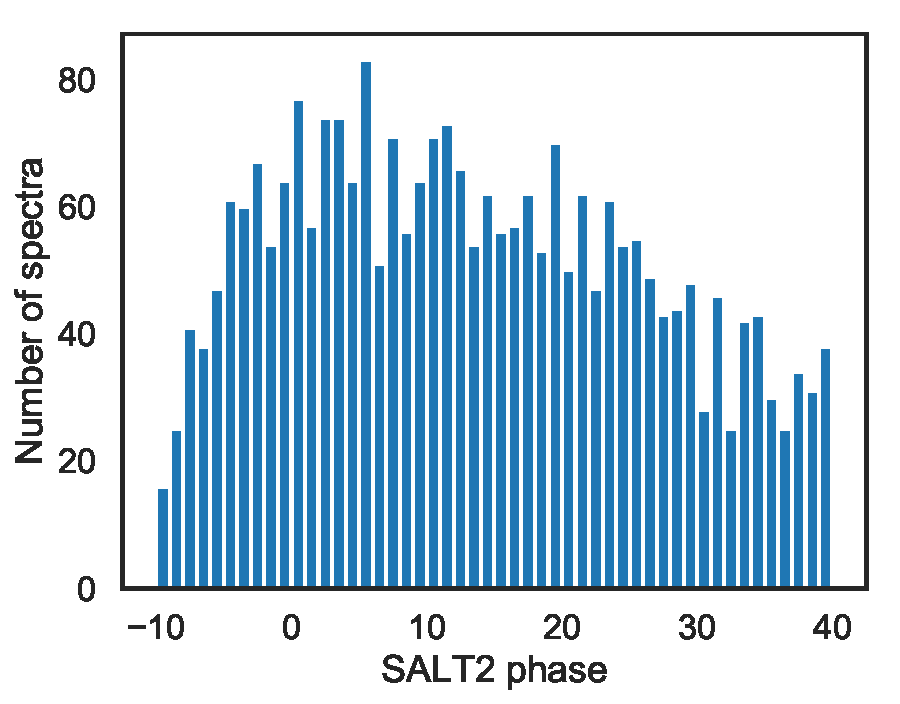
\includegraphics[width=0.5\textwidth]{figures/nn_twins/phase_histogram.pdf}
    \caption{Histogram of SALT2 phases for the complete data set. The phases are estimated from SALT2 fits to light curves synthesized from the full spectral time-series data of each supernova.}
    \label{fig:phase_distribution}
\end{figure}

These 2623 spectra serve as the inputs to the \stoe{} model. The labels are the phases determined from SALT2 fits to synthesized photometry, along with the per-supernova twins embedding coordinates $(\xi_1, \xi_2, \xi_3)$, magnitude offsets $\Delta m$, and relative dust extinction values $\Delta A_V$ from \citetalias{boone_twins_2020a}. For the \etos{} model, we use the normalized versions of these spectra (i.e. the spectra corrected for $\Delta m$ and $\Delta A_V$) as the labels for the network and the inputs are the corresponding embedding coordinates.

For the standardization analysis, \citetalias{boone_twins_2020b} uses a smaller subset of 173 \sne used to train the twins embedding in order to avoid errors from inaccurate host galaxy redshifts, peculiar velocities, and differences in dust properties. Thus, the standardization analysis in \citetalias{boone_twins_2020b} and our work uses only objects that have a quality host galaxy redshift, $z<0.02$, and $\Delta A_V < 0.5$. This subset consists of 134 objects.

\subsection{Training, Validation, and Test Sets and Cross-Validation}
\label{sec:nn_twins_data_split}
To avoid overtraining and ensure the generalizability of our models, we separated our data into training, validation, and test subsets. The sizes of these subsets are 142, 20, and 41 (70\%, 10\%, and 20\%) respectively. The supernovae were placed into each group randomly, and we ensured consistent placement in each group by fixing the pseudo-random generator seed in our analyses. We separated the data on a supernova-by-supernova basis rather than a spectrum-by-spectrum basis in order to avoid data leakage from e.g. spectra with multiple observations within a few nights.

During the hyperparameter tuning stage (Section \ref{sec:hyperparam}), we trained each model using the training set and evaluated its performance using the validation set. To ensure robustness to changes in the validation set, we performed 5-fold cross-validation on the combined training and validation sets to select the best hyperparameter combinations from the initial sweep. $k$-fold cross-validation is a commonly used model evaluation technique used for smaller data sets, wherein we split our data set into $k$ segments, train our model on $k-1$ of those segments and evaluate the trained model on the held-out segment. Using the average performance across these segments, we have a robust estimate of how well the predictions will generalize to unseen data sets. Once the hyperparameters were selected, we combined the training and validation sets (162 total \sne) to train the final models. The test set \sne where only used once all analysis steps were finalized.

This standard workflow of splitting data sets into training, validation, and test subsets is common in deep learning contexts because deep learning studies often operate in the regime where the size of the data set is extremely large and training an individual instance of the model is computationally expensive. However, in this work, we have a relatively small model trained on a fairly small data set. Cross-validation, like $k$-fold cross-validation, can help us to bolster the strength of our claims about out-of-sample performance by using a larger effective data set.

The logical extension of $k$-fold cross-validation is to set $k$ equal to the number of observations in the data set, a technique known as leave-one-out cross-validation (LOOCV). For every object in our data set, we train a separate model using data from every other object, then evaluate that model on the left-out object. This technique was used to evaluate the out-of-sample performance of the Gaussian process regression model used in \citetalias{boone_twins_2020b}, and we perform a similar final analysis to complete the comparison for our standardization study. This final study used the full data set (training, validation, and test) to perform LOOCV for both the \stoe{} embedding neural network training and the conditioning of the Gaussian process regression model.

\section{Models} \label{sec:model}
The models used in this analysis are multi-layer perceptrons (MLPs), simple artificial neural networks capable of capturing non-linear mappings from $m$-dimensional data to $n$-dimensional labels. Each network consists of several layers of nodes using either rectified linear unit (ReLU, \citet{nair_rectified_2010}) or $\tanh$ activation functions, with each layer fully connected to its neighboring layers.

The first model we explore, \stoe, takes a single deredshifted and rebinned spectrum of a supernova (see Section \ref{sec:nn_twins_data}) and predicts the phase of that spectrum, along with the relative extinction parameter $\Delta A_V$ and twins embedding coordinate $(\xi_1, \xi_2, \xi_3)$ of the supernova that the spectrum came from. This model allows us to use the \citetalias{boone_twins_2020b} standardization method on spectra at a wider range of phases. The second model, \etos, reverses this operation, taking an embedding coordinate and phase and producing a spectrum. This model can then be used for generating mock spectra for simulations, or for forward-model fitting to photometry. Both neural network models are implemented in \texttt{PyTorch} \citep{paszke_pytorch_2019}, and the full generative model of \etos{} is implemented as an \texttt{sncosmo} \texttt{Source} object \citep{barbary_sncosmo_2015}.

% A separate class of neural networks that are popular in many astronomical contexts is the convolutional neural network (CNN). CNNs use specialized convolutional layers that replace the matrix multiplication step of some of their layers with a kernel convolution. Doing so enables the networks to learn translation-invariant features of the input data, and stacking several convolutional layers enables the network to learn hierarchies of these features. This is a powerful technique for image classification tasks because images have an inherently hierarchical structure of salient features and the locations of where these features appear is not important to the final classification. \footnote{For example, low-level layers of a CNN may learn features like lines and dots and later layers may combine these features into eyes or sails, eventually learning some representation of dog or boat that can be used to detect such an object regardless of where the object is in the frame of a photograph.}

% However, we opted not to use this type of network specifically because of the translation-invariant structure imposed by CNNs. \cite{Boone2020a} found that some embedding dimensions correspond to specific spectral features located at particular wavelengths. The $\xi_1$ coordinate, for example, is associated with strong changes in the width of calcium features, but not similarly-shaped silicon or sulfur features. Additionally, $\xi_3$ is associated with varying ejecta velocities, imprinted in the spectra as a shift in the wavelength direction due to the Doppler shifting of the absorption profiles. Ideally, our network should be able to use this velocity shift as a differentiating feature, so a translation invariant network may be less efficient.

\subsection{Model Architecture and Hyperparameter Optimization}
\label{sec:hyperparam}
Selecting the optimal architecture of an MLP (i.e. the number of layers and the number of nodes per layer) remains an open field of research. The universal approximation theorem states that an MLP with a sufficiently large number of nodes in a single hidden layer is able to approximate any function with any desired error. In practice, however, meeting the ``sufficiently large hidden layer" criterion can be unfeasible, and though the network may be able to represent the function, the learning algorithms used to find the ideal weights may not be well-suited to ensure the learned weights produce this representation during training. Empirically, deep neural nets (i.e. MLPs with more than one hidden layer) have been shown to be more tractable solutions that generalize well after training \citep{goodfellow_deep_2016}.

The choice of activation function is also important. The ReLU activation function (linear for values greater than 0 and 0 otherwise) is empirically quite successful, due to its computational simplicity and properties that allow it to skirt the ``vanishing gradient" problem. ReLU also encourages the learned model weights to be sparse. However, this function is discontinuous, and can therefore cause the resulting outputs to be discontinuous as well. Discontinuity is acceptable in the \stoe{} model, since we make no a priori assumptions about the smoothness of the twins embedding space. For the \etos{} model, on the other hand, we know that our outputs should be smooth because we know that the evolution of spectra is smoothly varying. For this reason, we use the $\tanh$ activation function in the \etos{} model and the ReLU activation function in \stoe{}.

There are additional hyperparameters beyond the architectural design that we can include in the networks. Dropout layers \citep{srivastava_dropout_2014} can help to avoid overfitting and improve generalization, but the probability used to determine the number of connections to drop must be selected. The batch size (the number of training samples used in each training iteration) can also impact our results regardless of final architecture.

There are few strict rules governing the choice of these hyperparameters, so they are typically selected by experimentation. For our work, we used the Bayesian hyperparameter optimization framework implemented in the Weights and Biases package \citep[\texttt{wandb},][]{biewald_experiment_2020} to search over a range of potential model architectures and other hyperparameters (see Table \ref{tab:hyperparams}). For each combination of hyperparameters, we trained a model on our training data set, and evaluated the performance of the model by calculating the average mean squared error of the spectra in the validation set. These validation loss evaluations are then used to train a Gaussian process model in the hyperparameter space, and this model informs the choice of the next combination of hyperparameters to use in the sweep (see \citet{snoek_practical_2012}). The initial sweep used 239 trials for the \verb|spec2embedding| model and 252 trials for the \verb|embedding2spec| model (approximately 6 CPU-hours for each model, run serially). Each model was trained with 150 epochs -- enough to ensure convergence.

As explained in Section \ref{sec:nn_twins_data_split}, we perform 5-fold cross-validation on the top 10 best-performing models from this initial sweep to obtain a final model that is robust to variations in which supernovae end up in the validation set. The final model that we selected was the model with the lowest average cross-validation loss. The preferred hyperparameters from this second round of validation are also listed in Table \ref{tab:hyperparams}.

\begin{table}[htbp]
    \centering
    \begin{tabular}{lccc}\toprule
        \multirow{2}{*}[-1em]{Hyperparameter} &
        \multirow{2}{*}[-1em]{Value options} & \stoe{} & \etos\\
         & & preferred & preferred\\\midrule
        Network depth & [1, 2, 3, 4] & 3 & 4\\
        Nodes per layer & [72, 100, 128, 144, 172, 200, 228, 256, 288] & 256 & 144\\
        Dropout probability & [0, 0.001, 0.005, 0.01, 0.05, 0.1] & 0.001 & 0\\
        Batch size & [2, 4, 8, 16, 32] & 16 & 32\\\bottomrule
    \end{tabular}
    \caption{MLP hyperparameters values used in Bayesian optimization along with the preferred values for each model.}
    \label{tab:hyperparams}
\end{table}

We can see that a deeper architecture is preferred for both the \stoe{} and \etos{} models. This is consistent with the qualitative assessment that sequential network layers learn a hierarchical series of features. Both models also prefer smaller values for the dropout probability.

Using the hyperparameters in Table \ref{tab:hyperparams}, we performed our final training of the \stoe{} and \etos{} networks using the full combined training and validation sets. These are the final model weights used to evaluate the model accuracy on the held-out test set in Sections \ref{sec:spec2embed_results} and \ref{sec:embed2spec_results}.

\subsection{Magnitude Standardization Model}
The methodology for standardization given a twins embedding coordinate remains unchanged from the steps laid out in \citetalias{boone_twins_2020b}; we use the same Gaussian process (GP) regression model hyperparameters and minimally modify the training code. To condition the GP, we use the embedding coordinates and extinction parameters used in \citetalias{boone_twins_2020b} as input and the magnitude offsets found in the same work as output. We do not at this stage use the coordinates predicted by the \stoe{} model. As mentioned in Section \ref{sec:nn_twins_data}, we made the same selection cuts for standardization that are made in the \citetalias{boone_twins_2020b} analysis, removing objects that are very nearby ($z<0.02$), highly extincted ($A_V > 0.5$), with large uncertainties in redshift, or with poor data quality. This smaller subsample consists of 134 supernovae, 111 of which are in our combined training and validation set, and the remaining 23 are in our held-out test set.

Repeating the leave-one-out cross-validation analysis on the full data set yielded the same results as those presented in \citetalias{boone_twins_2020b}. To gather a baseline for a later standardization comparison, we used the same training process to condition the GP on the standardization training subset (111 \sne) and evaluated the model on the standardization test set (23 objects). We quantify our performance by calculating the residuals between the predicted values of $\Delta m$ and the values of $\Delta m$ found in \citetalias{boone_twins_2020a}, then measuring the RMS and normalized median absolute deviation (NMAD) of these residuals. The results from both the leave-one-out reproduction and the train-test split are summarized in Table \ref{tab:standardization_test_results}. Note that all of the embedding coordinate values used here are identical to those in \citetalias{boone_twins_2020b}; our intention is to examine how well the model performs on our smaller test set before we add in the additional uncertainty that comes from our neural network model. As expected, the results are all consistent with the leave-one-out cross-validation results, though the RMS values are slightly larger due to the smaller sample size.

Our analysis also differs from the \citetalias{boone_twins_2020b} analysis in that we are interested in building a model that can predict the supernova properties (like extinction and embedding coordinate) from multiple spectra. Thus, we also present the same measures of the spread in the per-supernova metrics weighted by the number of spectra that appear for those supernovae in our data set. The resulting values are all consistent with one another, but the error bars for the weighted values are smaller, reflecting the increase in the number of observations.

\begin{table}[htbp]
    \centering
    \begin{tabular}{rcccccc}\toprule
        & & & RMS & NMAD & Weighted RMS & Weighted NMAD\\
        Sample & $N_\textrm{SNe}$ & $N_\textrm{spec}$ & residuals (mag) & residuals (mag) & residuals (mag) & residuals (mag)\\\midrule
        Full sample LOO & 134 & 1683 & $0.102 \pm 0.008$ & $0.085 \pm 0.011$ & $0.105 \pm 0.002$ & $0.085 \pm 0.003$\\\midrule
        Training/val. & 111 & 1395 & $0.082\pm 0.007$ & $0.068\pm 0.009$ & $0.083\pm 0.002$ & $0.065\pm 0.002$\\
        Test & 23 & 288 & $0.120\pm 0.023$ &  $0.071\pm 0.025$ & $0.127\pm 0.006$ & $0.075\pm 0.007$\\
    \bottomrule
    \end{tabular}
    \caption{Summary of standardization results using the \citetalias{boone_twins_2020b} embedding coordinates and extinction parameters using our training and test sets. Weighted measures of the spread are weighted by the number of spectral observations for an individual supernova. All values are consistent with the values found in \citetalias{boone_twins_2020b}.}
    \label{tab:standardization_test_results}
\end{table}

% We trained an additional version of the GP regression model, conditioned on the \citetalias{Boone2020b} embedding coordinate values of \emph{all} of the supernovae in the standardization data set. This model can be used for a separate comparison to give us a sense of the size of the error stemming from directly propagating the error from the neural network predictions of the embedding coordinate to the error on the GP-predicted magnitude, without the additional error coming from the conditioning of the GP.

\subsection{Generating Spectra with \etos}
When training the \etos{} model, we used the deredshifted, rebinned, dereddened, and magnitude-normalized spectra as our model labels (see Section \ref{sec:nn_twins_data}). By doing so, the network only needs to learn the variation in the spectra due to changes in its phase and its parent supernova's location in the embedding space. The effects of differences in extinction and overall brightness can easily be added afterward. Mathematically, the deredshifted spectrum $f(\lambda)$ of a supernova with embedding coordinate ($\xi_1$, $\xi_2$, $\xi_3$), extinction $A_V$, and magnitude offset $\Delta m$ observed as phase $p$ is modeled as
\begin{equation}
    f(\lambda; p, \xi_1, \xi_2, \xi_3, A_V, \Delta m) = \texttt{embed2spec}(p, \xi_1, \xi_2, \xi_3) \times 10^{0.4 [\text{F99}(\lambda; A_V, R_V=2.8) + \Delta m]}
    \label{eqn:etos_flux}
\end{equation}
where $\text{F99}(\lambda; A_V, R_V=2.8)$ is the extinction-color relation of \citet{fitzpatrick_correcting_1999} using a total-to-selective extinction ratio of $R_V=2.8$. Using Equation \ref{eqn:etos_flux}, we can then easily synthesize lower-resolution or broadband photometric observations, enabling forward modeling fits to these alternate data types.

\section{\stoe{} Results}
\label{sec:spec2embed_results}
\subsection{Recovering Phase, Extinction, and Twins Embedding Coordinates}
Using the final trained \stoe{} model, we now evaluate its performance on the test set that has thus far been completely unseen by the model. Figure \ref{fig:scatter_spec2embed_phase_color} shows the predicted phases and extinction parameters as a function of the true phases and extinction parameters, and Figure \ref{fig:scatter_spec2embed_coords} shows the same for each of the twins embedding coordinates $(\xi_1, \xi_2, \xi_3)$. Using the NMAD of the residuals to measure our accuracy, we find that the model is able to constrain the phase of the spectrum to within $\pm 2.4$ days, the extinction to within $\pm 0.1$ mag, and the embedding coordinates to within $0.69$, $0.52$, and $0.59$ for $\xi_1$, $\xi_2$, and $\xi_3$ respectively.

\begin{figure}
    \centering
    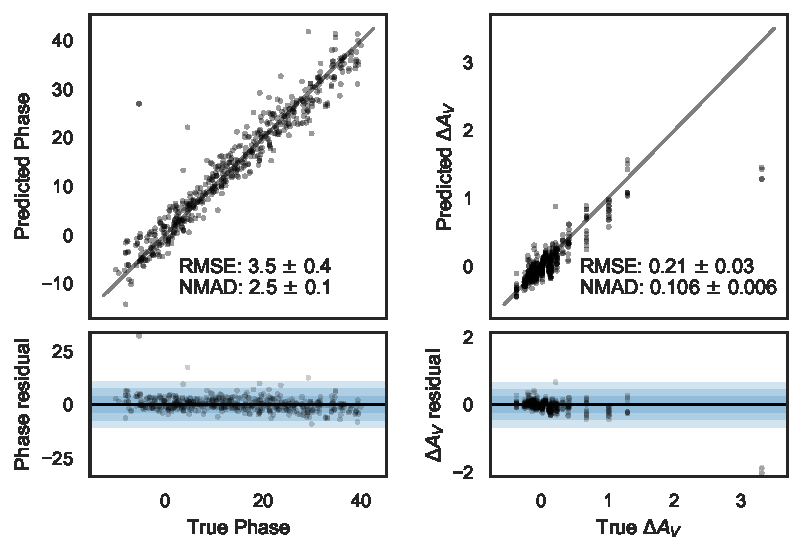
\includegraphics[width=0.9\textwidth]{figures/nn_twins/scatter_spec2embed_phase_color.pdf}
    \caption{Comparison of phase and extinction parameters determined by the \stoe{} model and ground truth values presented in \citetalias{boone_twins_2020a}. The solid lines in each of the upper panels represents equivalence. We also note the root-mean-squared-error (RMSE) and the normalized median absolute deviation (NMAD) of the residuals (predicted value $-$ true value) for each property. The lower panels show these residuals as a function of the true values. Shaded regions in the lower panels indicate the 1-, 2-, and 3-$\sigma$ fluctuations of these residuals about the median.}
    \label{fig:scatter_spec2embed_phase_color}
\end{figure}

\begin{figure}
    \centering
    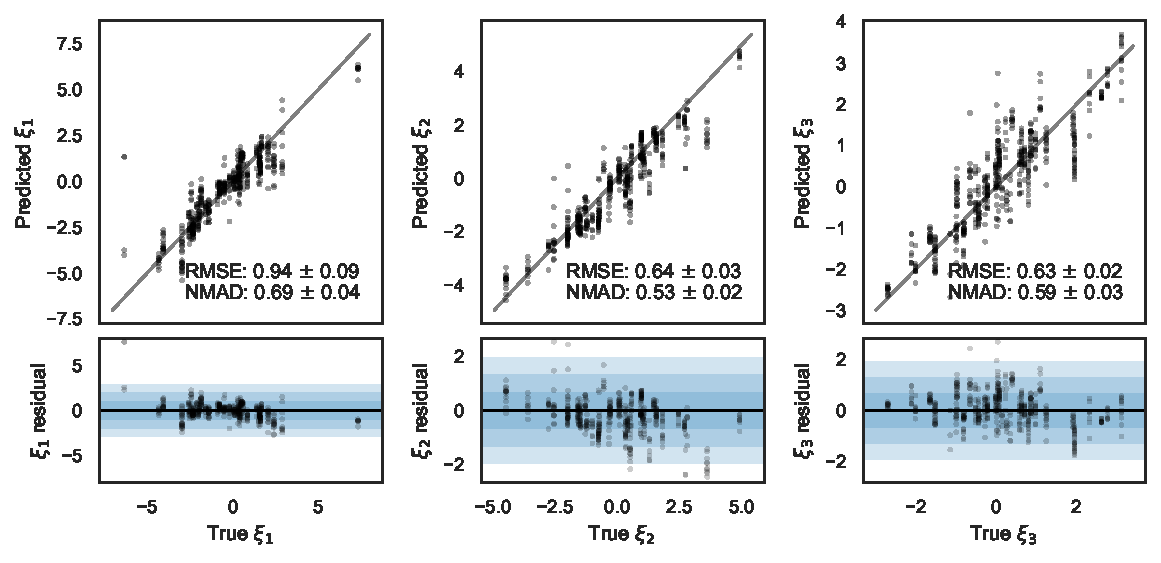
\includegraphics[width=0.9\textwidth]{figures/nn_twins/scatter_spec2embed_coords.pdf}
    \caption{Same as Figure \ref{fig:scatter_spec2embed_phase_color}, but comparing the predicted and ground-truth twins embedding coordinates $\xi_1$, $\xi_2$, and $\xi_3$.}
    \label{fig:scatter_spec2embed_coords}
\end{figure}

The phase recovery is slightly more accurate than the commonly used SNID program \citep{blondin_determining_2007}, which can constrain the phase to within $\pm 2.9$ days. It is not quite as accurate as other neural network based techniques like \citet{stahl_deepsip_2020}, which constrains the phase to with $\sim\pm 1$ day. Even in the restricted phase baseline of -4 to +12 days beyond maximum brightness that is used in \citet{stahl_deepsip_2020}, we have an NMAD of the residuals of 2.4 days. However, as we will see in Section \ref{sec:standardization} that the phase determination is not as important for standardization as the accuracy in determining the extinction and location in the twins embedding space of each object. 

The accuracy in determining the extinction parameter is sufficient for standardization, as a 0.1 mag error in $\Delta A_V$ propagates to a 0.015 mag error in the final standardized brightness. There is one large outlier in color in our test set: SN2006X. This object is highly extincted ($\Delta A_V=3.31$), more so than the most highly extincted object in the training set (SN2012cu, $\Delta A_V=2.8$). Both of these highly extincted objects are excluded from the standardization analysis to avoid biases from uncertainties in interstellar dust properties, so the errors here do not propagate to the standardization analysis.

\subsection{Standardization Results} 
\label{sec:standardization}
We now use the Gaussian process regression model conditioned on the true embedding coordinates and extinction parameters of the training and validation sets to make predictions of the magnitudes based on the embedding coordinates that were predicted by the trained \stoe{} network. The results are summarized in Table \ref{tab:standardization_nn_results}. The first results column is identical to the weighted results of Table \ref{tab:standardization_test_results}, since the results are weighted on a spectrum-by-spectrum basis rather than a supernova-by-supernova basis.

Because the embedding predictions for the training set are so similar to the ground truth predictions, the resulting predictions for the standardized magnitudes are also very similar (differing on average by less than 0.01 mag). The test set gives us a better sense of how well this method of standardization will perform on outside data, as all of the observations of these objects were unseen in both the neural network training and the standardization model conditioning. Here, we see a slight inflation in the errors; on average the error in the embedding coordinate prediction propagates to an 0.024 magnitude error in the standardized brightness. This is however subdominant to the standardization model error, indicating that these neural-network-predicted embedding coordinates at all phases can be used about as successfully as the RBTL and Isomap fits from maximum brightness spectra.

\begin{table}[htbp]
    \centering
    \begin{tabular}{rrcc}\toprule
    \multicolumn{2}{c}{Metric} & Training & Test\\
    \multicolumn{2}{c}{} & Single epoch & Single epoch\\\midrule
    \multicolumn{2}{c}{$N$} & 1395 & 288\\\midrule 
    $\textrm{GP}(\textrm{true}) - \Delta m_\textrm{true}$ & RMS & 
        $0.083\pm 0.002$ & $0.127\pm 0.006$\\
    & Pec. vel. removed &
        $0.064\pm 0.003$ & $0.110\pm 0.007$\\
    & NMAD & 
        $0.064\pm 0.003$ & $0.083\pm 0.010$\\
     $\textrm{GP}(\textrm{pred}) - \Delta m_\textrm{true}$ & RMS & 
        $0.085\pm 0.002$ & $0.130\pm 0.006$\\
    & Pec. vel. removed & 
        $0.066\pm 0.003$ & $0.114\pm 0.007$\\
    & NMAD & 
        $0.068\pm 0.003$ & $0.087\pm 0.008$\\\midrule
     $\textrm{GP}(\textrm{pred}) - \textrm{GP}(\textrm{true})$ & RMS & 
        $0.009\pm 0.0003$ & $0.024\pm 0.001$\\
    & NMAD & 
        $0.008\pm 0.0002$ & $0.021\pm 0.002$\\\bottomrule
    \end{tabular}
    \caption{Standardization errors for the training and test data sets using the Gaussian process regression model conditioned on the \citetalias{boone_twins_2020a} embedding coordinates to predict the absolute magnitudes based on the \citetalias{boone_twins_2020a} embedding coordinates and the \stoe{} neural-network predicted embedding coordinates, as well as the average difference between these predictions. Errors on the statistics are determined via bootstrap resampling.}
    \label{tab:standardization_nn_results}
\end{table}

In Figure \ref{fig:stand_err_vs_phase}, we show the NMAD of the differences between the standardized magnitudes predicted from the  \stoe-predicted embedding coordinates and the magnitudes predicted form the true embedding coordinates (i.e. $\textrm{GP}(\textrm{pred}) - \textrm{GP}(\textrm{true})$ in Table \ref{tab:standardization_nn_results}) as a function of the spectrum phase for the test set. The spread of the errors is roughly consistent across phases, providing further credence to the claim that the neural network gives us the ability to standardize across a wide range of phases. The large error in the first phase bin (-10 to -7.5 days) is driven mainly by the paucity of test data in this region.

\begin{figure}[htbp]
    \centering
    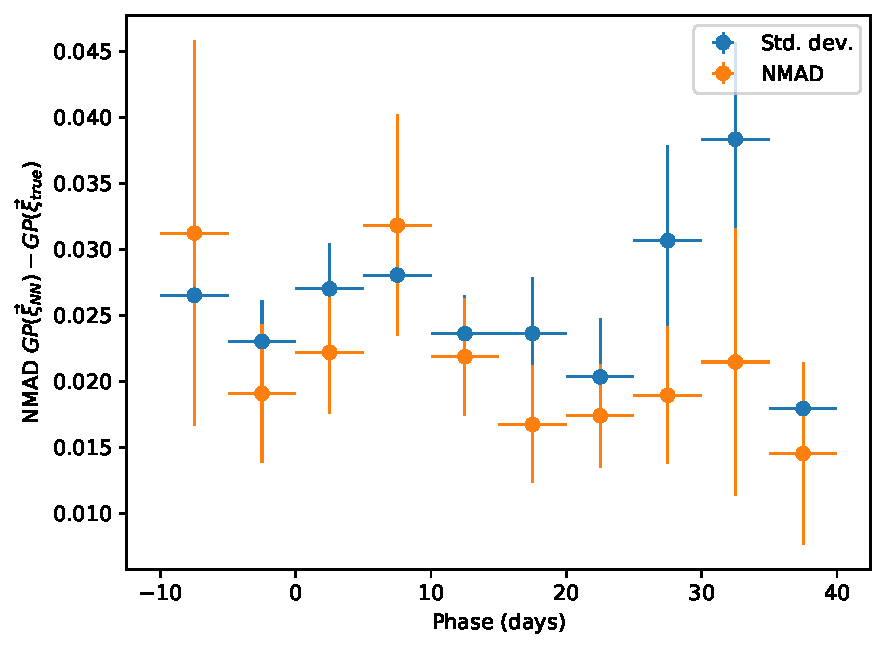
\includegraphics[width=0.9\textwidth]{figures/nn_twins/stand_err_vs_phase_nn.pdf}
    \caption{NMAD of the difference between the magnitudes predicted from the neural network predicted embeddings and those predicted from the true embeddings as a function of the spectral phase.}
    \label{fig:stand_err_vs_phase}
\end{figure}

\subsection{Leave-One-Out Analysis}
Our claims about how well this technique is able to standardize \sne are perhaps limited by the small size of our test set. In order to make our claims more precise, as well as to have a fair comparison with the standardization results of \citetalias{boone_twins_2020b}, we perform a full leave-one-out cross-validation analysis of both the neural network training and the GP regression conditioning. We used the complete data set of 203 supernovae to train 203 instances of the \stoe{} model, each using the data from all but one supernova. We performed a similar analysis, training 134 versions of the GP regression model using the embedding coordinates from \citetalias{boone_twins_2020b}. When evaluating the standardization by combining the two models, we ensure that the same supernova was held out in both models.

In Figures \ref{fig:scatter_spec2embed_loo_phase_color} and \ref{fig:scatter_spec2embed_loo_coords}, we show the comparison of the true phases, extinctions, and embedding coordinates from this leave-one-out test for the entire data set. The spreads of the residuals are all roughly similar to their values for the smaller test set, and we present an explicit comparison in Table \ref{tab:loocv_comparison}.

In Table \ref{tab:standardization_loo_results}, we summarize the size of the standardization errors as determined by this full leave-one-out analysis. We find that with our neural network model, we can standardize supernova magnitudes with a precision comparable to the near-maximum twins embedding analysis, even when using spectra far from maximum brightness. We can see this more clearly in Figure \ref{fig:stand_err_vs_phase_loo}, where we show the NMAD of the LOOCV magnitude residuals as a function of phase. Again, the large error bar in the -10 day to -7.5 day bin is due to how few spectra there are available in that window. We can also see in this figure that our single spectrum standardization method surpasses the standardization power of the commonly used SALT2 model, which requires the observation of a full broadband light curve.  

\begin{figure}
    \centering
    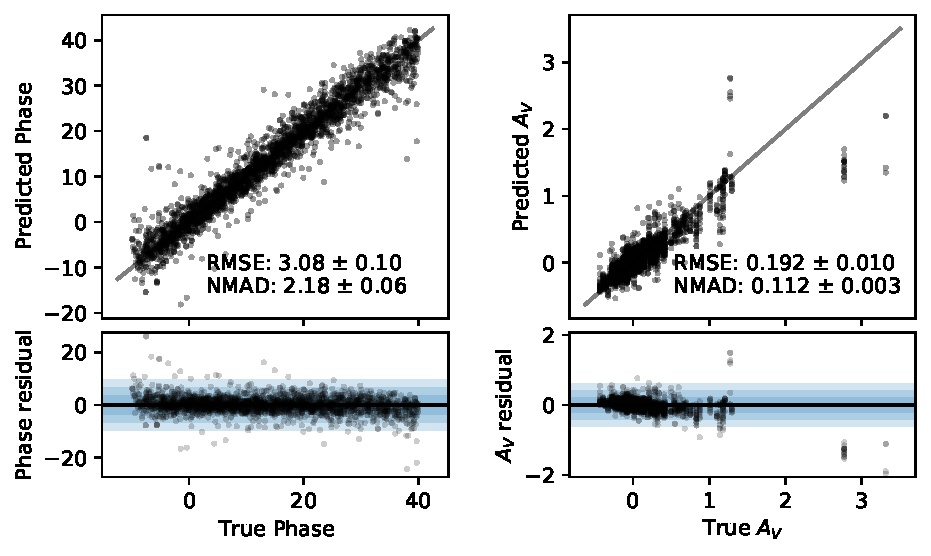
\includegraphics[width=0.9\textwidth]{figures/nn_twins/scatter_loo_spec2embed_phase_color.pdf}
    \caption{Same as Figure \ref{fig:scatter_spec2embed_phase_color}, but using the leave-one-out cross-validation analysis. As in Figure \ref{fig:scatter_spec2embed_phase_color}, each point represents a single spectrum. However, the predictions are made using networks trained on every supernova except the supernova the spectrum comes from.}
    \label{fig:scatter_spec2embed_loo_phase_color}
\end{figure}

\begin{figure}
    \centering
    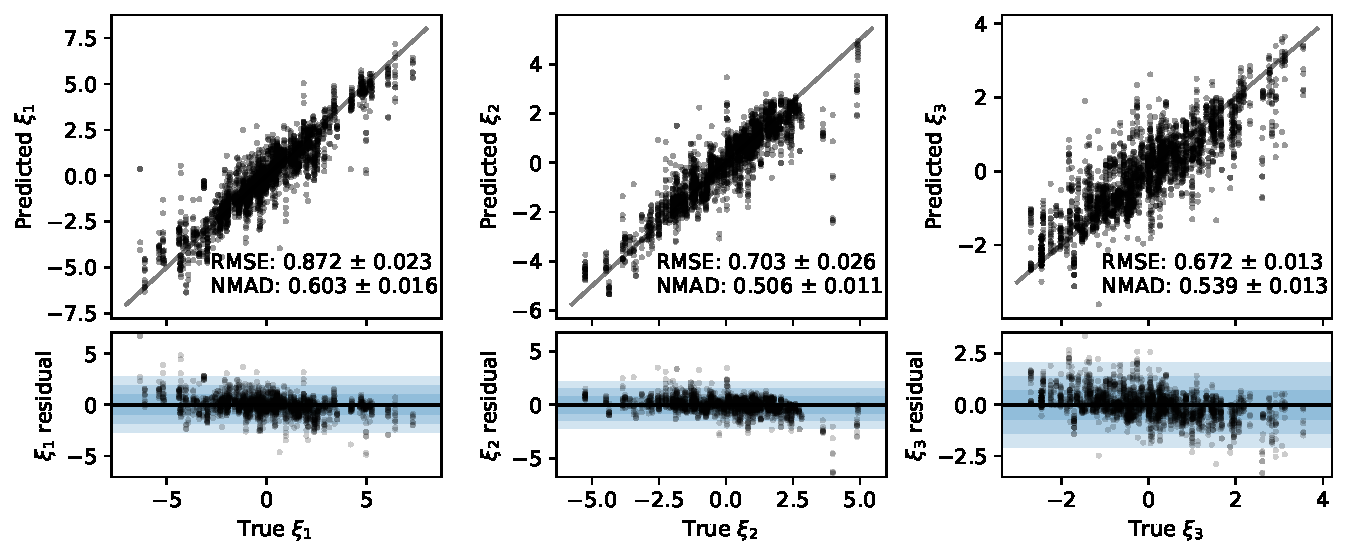
\includegraphics[width=0.9\textwidth]{figures/nn_twins/scatter_loo_spec2embed_coords.pdf}
    \caption{Same as Figure \ref{fig:scatter_spec2embed_loo_phase_color}, but for the embedding coordinates.}
    \label{fig:scatter_spec2embed_loo_coords}
\end{figure}

\begin{table}[htbp]
    \centering
    \begin{tabular}{cccc}\toprule
        Parameter & Metric & Test set & LOOCV \\\midrule
        Phase & RMS & $3.5 \pm 0.4$ & $3.0 \pm 0.10$ \\
        & NMAD & $2.48 \pm 0.12$ & $2.18 \pm 0.06$\\
        $\Delta A_V$ & RMS & $0.21 \pm 0.04$ & $0.192 \pm 0.010$ \\
        & NMAD & $0.106 \pm 0.007$ & $0.112 \pm 0.003$\\
        $\xi_1$ & RMS & $0.95 \pm 0.09$ & $0.87 \pm 0.02$ \\
        & NMAD & $0.70 \pm 0.04$ & $0.60 \pm 0.02$\\
        $\xi_2$ & RMS & $0.65 \pm 0.03$ & $0.70 \pm 0.03$ \\
        & NMAD & $0.52 \pm 0.02$ & $0.506 \pm 0.011$\\
        $\xi_3$ & RMS & $0.64 \pm 0.02$ & $0.672 \pm 0.013$ \\
        & NMAD & $0.60 \pm 0.03$ & $0.539 \pm 0.013$\\
        \bottomrule
    \end{tabular}
    \caption{Comparison of parameter accuracy between the test set evaluation in Section \ref{sec:spec2embed_results} and the LOOCV evaluations.}
    \label{tab:loocv_comparison}
\end{table}

\begin{table}[htbp]
    \centering
    \begin{tabular}{crc}\toprule
        \multicolumn{2}{c}{Metric} & LOOCV value \\\midrule
        $\textrm{GP}(\textrm{true}) - \Delta m_\textrm{true}$ & RMS & $0.105 \pm 0.002$ \\
        & Pec. vel. removed & $0.089 \pm 0.003$\\
        & NMAD & $0.085 \pm 0.003$ \\
        $\textrm{GP}(\textrm{pred}) - \Delta m_\textrm{true}$ & RMS & $0.107 \pm 0.002$ \\
        & Pec. vel. removed & $0.092 \pm 0.003$ \\
        & NMAD & $0.092 \pm 0.003$\\
        $\textrm{GP}(\textrm{pred}) - \textrm{GP}(\textrm{true})$ & RMS & $0.0327\pm 0.0012$\\
        & NMAD & $0.0220 \pm 0.0008$\\
    \bottomrule
    \end{tabular}
    \caption{Standardization results using a full leave-one-out cross-validation analysis. Each measure of the spread was obtained by training a separate \stoe{} model and GP regression model for each supernova, where both models are conditioned on the data from all SNe except that held-out SN. Uncertainties on the values of these metrics were determined via bootstrap resampling.}
    \label{tab:standardization_loo_results}
\end{table}

\begin{figure}
    \centering
    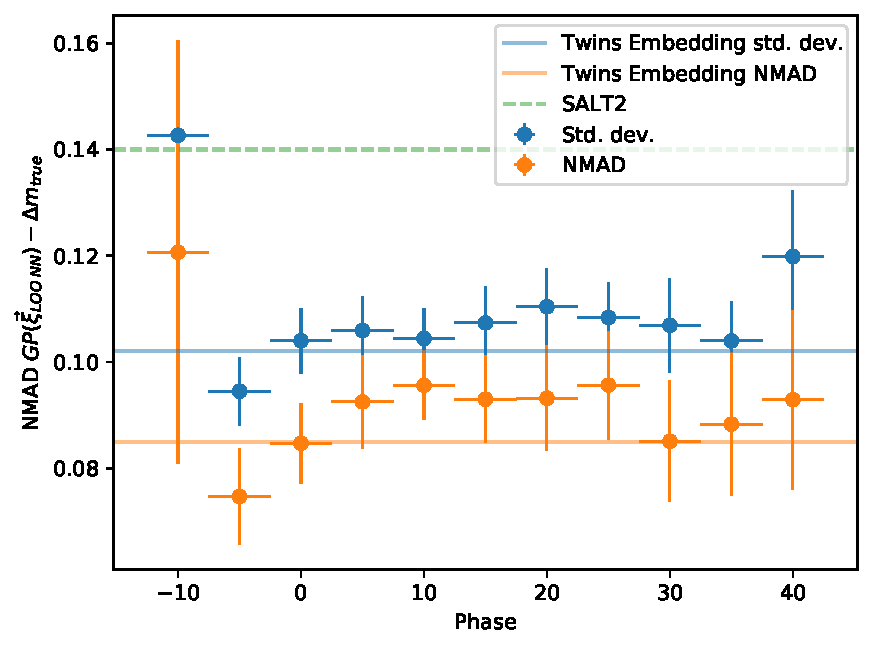
\includegraphics[width=0.9\textwidth]{figures/nn_twins/stand_err_vs_phase_loo.pdf}
    \caption{NMAD of the standardization residuals ($\textrm{GP}(\textrm{pred}) - \Delta m_\textrm{true}$) as a function of phase for the full leave-one-out cross-validation analysis. We also show the value of this metric for the twins embedding analysis, as well as for the SALT2 model.}
    \label{fig:stand_err_vs_phase_loo}
\end{figure}

\section{Recovering Spectra with \etos}
\label{sec:embed2spec_results}
The \etos{} model allows us to extend the twins embedding into a generative model that can then be used to fit other types of observations, like photometric light curves. We have implemented a version of the trained model as a \texttt{Source} object in \texttt{sncosmo}, a Python package for supernova cosmology. This allows us to easily add the effects of redshifting and dust extinction, as well as providing methods for synthesizing photometry.

To get a qualitative sense of the performance of this model, we show some example reconstructions. In Figure \ref{fig:PTF09dnl_spec}, we compare the observed spectral time-series data for PTF09dnl, a supernova in our held-out test set, to the spectra time-series predicted by \etos. Figure \ref{fig:PTF09dnl_lc} shows a similar comparison using synthesized photometry in top-hat band passes corresponding roughly to Bessell BVRI bands (Table \ref{tab:snf_tophats}). The observed and predicted data align fairly well, though at earlier phases, the agreement is less strong, particularly near the CaII H\&K feature from 3500 to 3990 \AA.

\begin{figure}
    \centering
    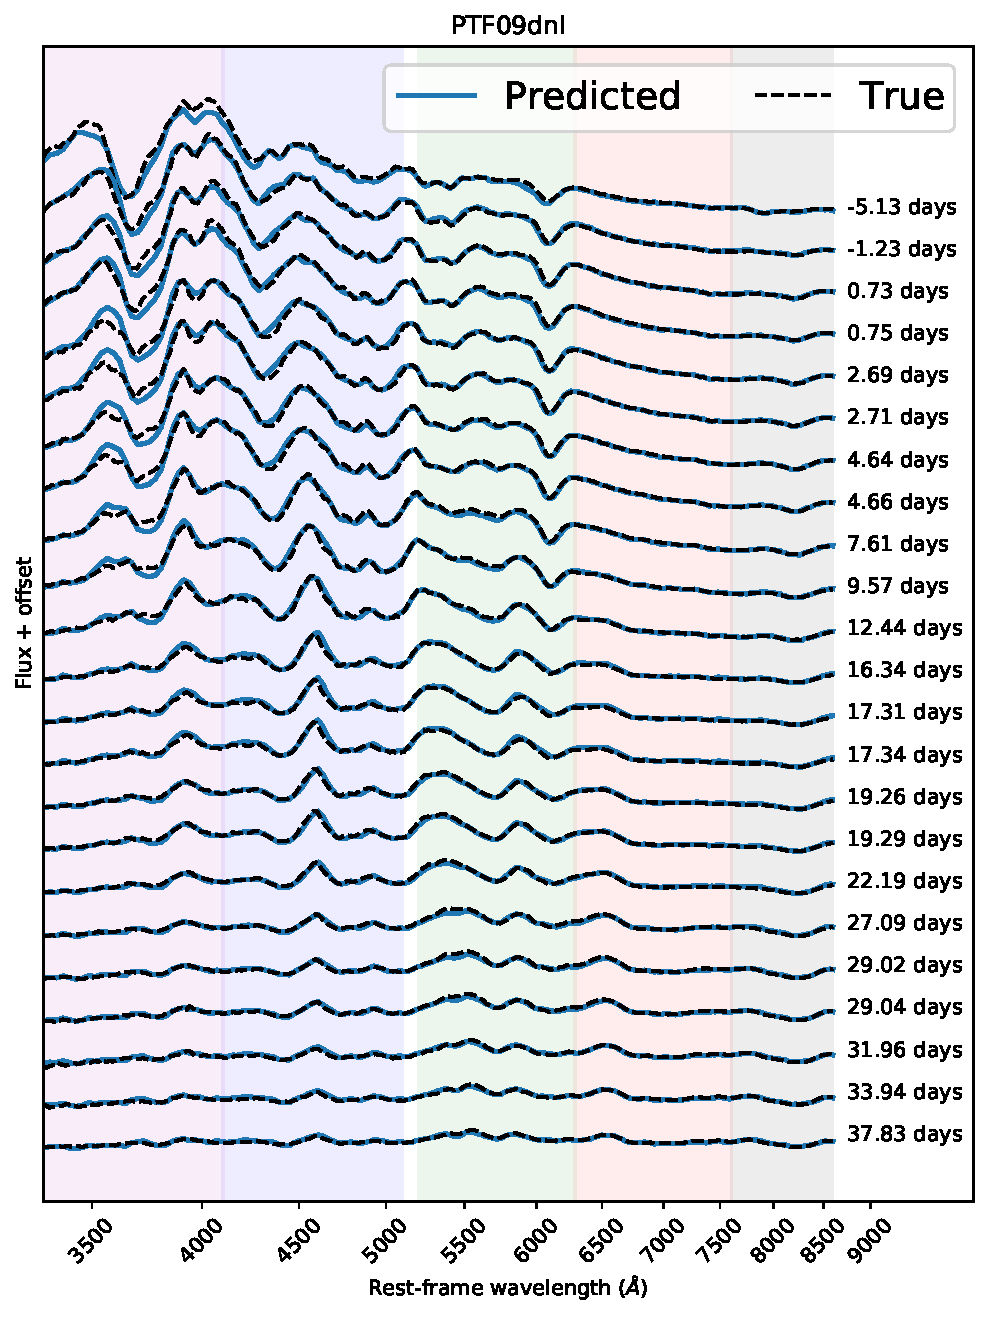
\includegraphics[width=0.85\textwidth]{figures/nn_twins/PTF09dnl_embed2spec.pdf}
    \caption{Comparison of the observed spectral time-series data (in black dashed lines) to the predicted data (blue solid lines) for PTF09dnl, a supernova in our held-out test set.}
    \label{fig:PTF09dnl_spec}
\end{figure}

\begin{figure}
    \centering
    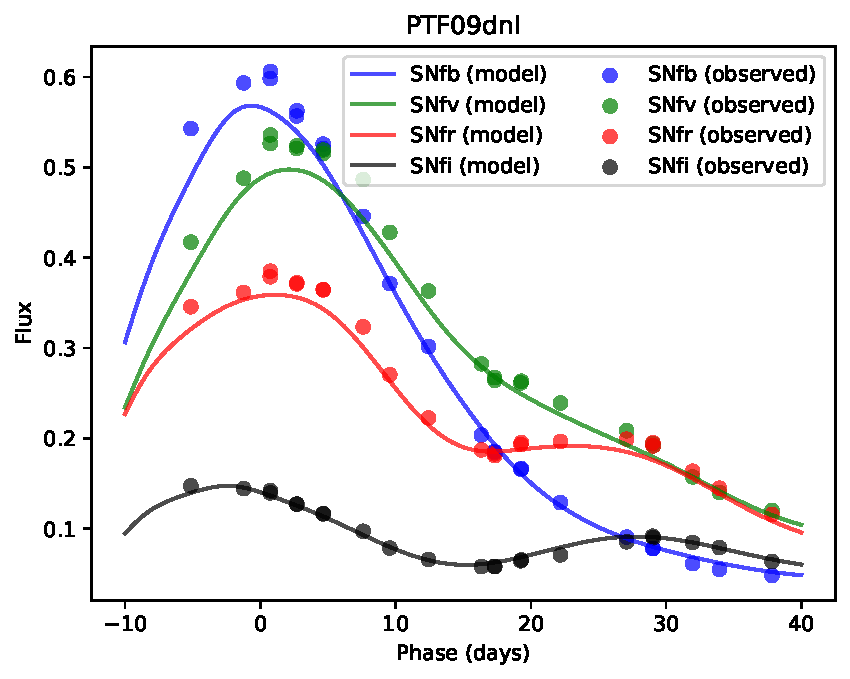
\includegraphics[width=0.9\textwidth]{figures/nn_twins/PTF09dnl_lc.pdf}
    \caption{Similar to Figure \ref{fig:PTF09dnl_spec}, but using synthesized photometry to compare the observer-frame light curves (dots) to the model predictions (solid lines). The band passes used are defined in Table \ref{tab:snf_tophats}.}
    \label{fig:PTF09dnl_lc}
\end{figure}

\begin{table}[htpb]
    \centering
    \begin{tabular}{cc}\toprule
        Name & Wavelength range (\AA) \\\midrule
        SNfu & (3300, 4102)\\
        SNfb & (4102, 5100)\\
        SNfv & (5200, 6289)\\
        SNfr & (6289, 7607)\\
        SNfi & (7607, 8600)\\\bottomrule
    \end{tabular}
    \caption{Top-hat band pass definitions.}
    \label{tab:snf_tophats}
\end{table}

We also examined the performance of this model over the full test set more quantitatively. For each spectrum of the supernovae in the test set, we calculated the flux residuals: the difference between the observed and predicted values. In Figure \ref{fig:e2s_wavelength_resids} we show the RMS of these residuals as a function of wavelength bin, normalized by the average flux in each wavelength bin marginalized over all observed phases. Between 4000 and 8000 \AA, the normalized RMS remains below 0.2 across all phases, indicating that the model is able to capture the flux to within 20\%. There are a few regions of the spectrum that have larger relative dispersions in the flux residuals -- these each correspond to well-known spectral features like the \ion{Ca}{2} H\&K doublet, the \ion{Si}{2} 6355~\AA\ line, the O triplet, and the \ion{Ca}{2} IR triplet. These features are also identified in \citetalias{boone_twins_2020a} as regions of higher variability near maximum brightness, which may contribute to this wider spread. Away from these regions, the spread of the residuals is at the 5-10\% level.

\begin{figure}
    \centering
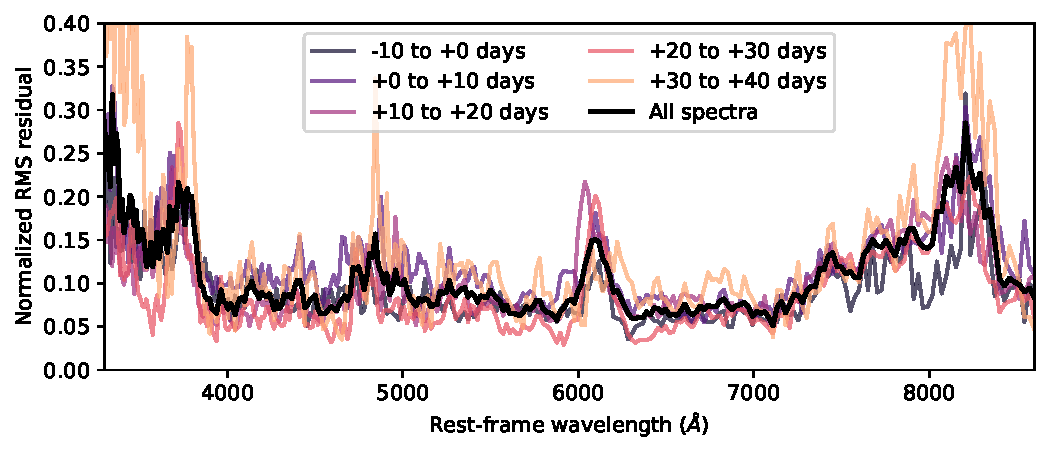
\includegraphics[width=0.9\textwidth]{figures/nn_twins/embed2spec_rms_wavelength.pdf}
    \caption{RMS of \etos{} flux residuals in each wavelength bin, normalized by the average flux in the bin across all phases. The thick black line shows the overall normalized RMS flux residual, and the thinner colored lines show the normalized RMS flux residual for subgroups selected by phase.}
    \label{fig:e2s_wavelength_resids}
\end{figure}

In addition to quantifying the model accuracy as a function of wavelength, we measure the performance as a function of phase. In Figure \ref{fig:e2s_phase_resids}, we plot the RMS of the flux residuals, normalized by the average flux for each spectrum as a function of the spectrum phase (after marginalizing over all wavelengths). As we may have anticipated, the errors are lowest near-maximum brightness, as there is less interpolation error and greater spectral coverage. Most of the larger outlying points correspond to spectra of SN2009hs and LSQ12fhs, two peculiar supernovae with subtypes that little representation in the training set (SN1991bg-like and SN2002cx-like, respectively). Excluding these two objects, our model is able to capture the spectrum flux to within approximately 20\% at all phases between $-10$ and $+30$ days after maximum brightness.

\begin{figure}
    \centering
    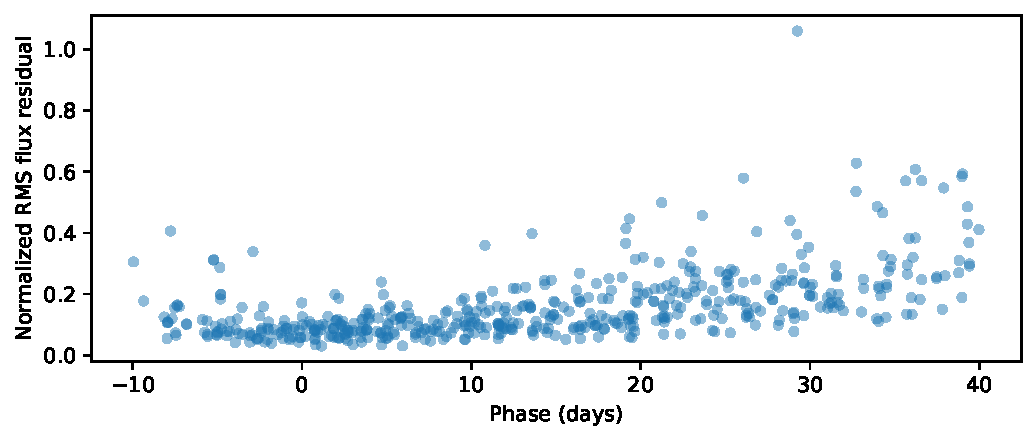
\includegraphics[width=0.9\textwidth]{figures/nn_twins/embed2spec_rms_phase.pdf}
    \caption{RMS of the flux residuals normalized by the average flux over all wavelengths at each phase. Most of the outlying points belong to either SN2009hs, a 91bg-like peculiar supernova, or LSQ12fhs, an 02cx-like peculiar supernova. Some outliers}
    \label{fig:e2s_phase_resids}
\end{figure}

Finally, we examine the fidelity of the \etos{} network results as a function of location in the twins embedding space. Figure \ref{fig:e2s_embedding_resids} shows the location of each test set supernova in the twins embedding space colored by its average normalized RMS flux residual. We can see that the supernovae that the model performs most poorly on are the objects on the periphery of the embedding space. The two largest outliers, SN2009hs and LSQ12fhs, are also made apparent in this plot. These peculiar subclasses of objects are not very well-represented in the training set (two 91bg-like objects and a single 02cx-like object), so this is unsurprising. Retraining this network with more observations of peculiar objects could further refine this work.

\begin{figure}
    \centering
    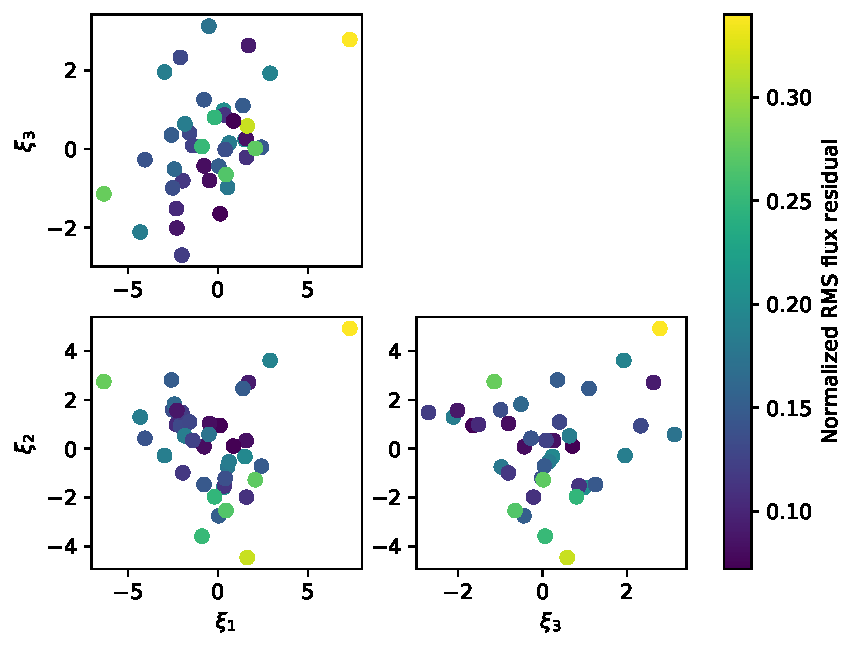
\includegraphics[width=0.9\textwidth]{figures/nn_twins/embed2spec_rms_embedding.pdf}
    \caption{Phase-averaged RMS flux residual for all observed spectra for each test set supernova as a function of twins embedding space coordinate.}
    \label{fig:e2s_embedding_resids}
\end{figure}

\section{Conclusions} \label{sec:nn_twins_conclusions}
We have presented an extension of the twins embedding analyses of \citetalias{boone_twins_2020a} and \citetalias{boone_twins_2020b} allowing the use of a wider range of phases to standardize Type Ia supernovae for cosmology. Our \stoe~model can predict the phase, relative extinction, and location in the twins embedding space of a \sn using any photometrically calibrated spectrum from $-10$ to $+40$ days after maximum brightness with high fidelity. Using these neural network predicted extinction and embedding coordinates, we can use the standardization model from \citetalias{boone_twins_2020b} to predict the absolute brightness of a supernova from any of its spectra with an RMS error of $0.107 \pm 0.002$ mag. If we account for peculiar velocities, this RMS error shrinks to $0.092 \pm 0.003$ mag. This standardization error is comparable to what was found using near-maximum spectra in \citetalias{boone_twins_2020b}, and is far superior to the error we can obtain using light curve based techniques like SALT2.

Additionally, we have trained and evaluated a separate model, \etos, which capable of generating spectral time-series data based on an embedding coordinate. This model can be used in simulations and in forward modeling fitting approaches, potentially allowing us to obtain the twins embedding coordinate of a supernova from more readily available photometry or lower-resolution spectroscopy.

There are a number of studies that may be done to extend this work even further. We have not yet studied how robust this model is to noise or made an attempt to quantify the accuracy of the forward-modeling approach of \etos{} as a function of spectral signal-to-noise ratio or resolution. The \stoe{} model requires a photometrically calibrated spectrum with sufficient resolution and wavelength coverage to create the binned, deredshifted spectra similar to those used in training. Many spectrographs do not have the level of calibration precision available with SNIFS. Using data augmentation techniques may prove useful in improving the results of the model \citep{boone_avocado_2019} and inuring the model from biases or errors stemming from calibration errors, lower signal-to-noise, or differences in wavelength coverage. Retraining the network with spectra preprocessed similarly the spectra used in e.g. \citet{stahl_deepsip_2020} may also allow us to use these same techniques while relaxing the spectrophotometricity constraint.

However, even without these additional studies, we have already produced a method for standardizing Type Ia supernova magnitudes with only a single spectrum observed anywhere within a wide range of phases. Moreover, the precision of this standardization is dramatically better than light curve-based techniques that require several observations. Spectra with the calibration necessary to use this technique are already obtainable. This technique may prove powerful in studies of the growth of structure via peculiar velocity measurements, or in measurements of the Hubble constant.

All software and data used in this analysis has been made publicly available on Github: \url{https://github.com/sam-dixon/nn_twins_embedding}.
